\documentclass[12pt, titlepage]{article}

\usepackage[utf8]{inputenc}
\usepackage[T1]{fontenc}
\usepackage[francais]{babel}
%\usepackage{Times}

%Mise en page

\usepackage[top=2cm, bottom=2.5cm, left=4cm , right=3cm]{geometry}
\usepackage{setspace}
%\setlength{\parskip}{1ex plus 0.5ex minus 0.2ex}

\usepackage{titlesec}
\titlespacing{\section}{0cm}{1cm}{1cm}
\titlespacing{\subsection}{0cm}{0cm}{0.5cm}

%Caractères spéciaux

\usepackage{lmodern}
\usepackage{amsmath}
\usepackage{amssymb}
\usepackage{mathrsfs}

\usepackage{eurosym} %insertion signe euro
\usepackage{graphicx} %insertion d'images
\usepackage{fancyhdr} %en-tete et pied de page
\usepackage{hyperref}%lien url

\title{\bsc{Rapport de projet}\\Projet flight arena}
\author{mr cube :\\
Vincent \bsc{Rospini Clerici} (rospin\_v),\\
Guillaume \bsc{Rebut} (rebut\_g)\\
chef de projet : Arthur \bsc{Remaud} (remaud\_a)}
\date{16 juin 2015}

\pagestyle{fancy}
\fancyhead{}
\fancyfoot{\thepage}
\lhead{\leftmark}
\rhead{Projet Flight Arena}
\lfoot{}
\rfoot{}


\begin{document}
\begin{spacing}{1.5}

%\maketitle

\begin{titlepage}

\begin{flushright}

\includegraphics[height=4cm, width=6cm]{logo-epita.png}\\[2cm]
\end{flushright}

\begin{center}
\textsc{\LARGE \bsc{Rapport de projet :}}\\[1.5cm]

\textsc{\Large Projet flight arena}\\
\textsc{du groupe mr cube}\\[1.5cm]

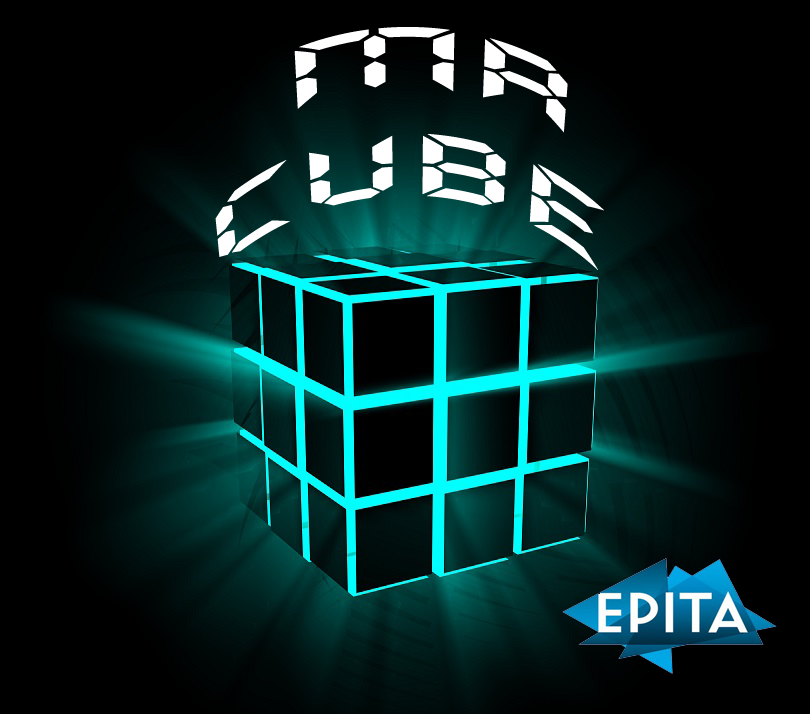
\includegraphics[height=6cm, width=6cm]{MRCUBE.png}\\[1cm]

\begin{flushleft}
Vincent \bsc{Rospini Clerici} (rospin\_v),\\
Guillaume \bsc{Rebut} (rebut\_g)\\
chef de projet : Arthur \bsc{Remaud} (remaud\_a)
\end{flushleft}

\begin{flushright}
1\ier{} année de classe\\ préparatoire intégrée
\end{flushright}

\vfill{16 juin 2015}
\end{center}
\end{titlepage}

\section*{Remerciements}
Nous souhaitons remercier l'école \bsc{Epita} qui nous a fourni le matériel dont nous avions besoin pour aboutir à ce projet. Notamment les ordinateurs disponibles 24/24 heures dans les locaux de l'école comprenant la majorité des logiciels nécessaires a la conception du jeu.\\

Nous souhaitons également remercier un de nos ami, Augustin Ledanseur sans qui la bande son originale du jeu n'aurait définitivement pas vu le jour. \\

\newpage

\renewcommand{\contentsname}{Sommaire}
\renewcommand{\chaptername}{Partie}

\tableofcontents
\addcontentsline{toc}{section}{Introduction}


\newpage
\section*{Introduction}
Le groupe mr cube, composé de Guillaume Rebut, Vincent Rospini Clerici et Arthur Remaud, est fier de vous présenter son projet : \textit{flight arena}.\\

Ce projet est réalisé dans le cadre  du projet de première année de l'école \bsc{Epita}. C’est un projet libre par groupe de quatre. Le but est de nous apprendre à travailler en équipe, tout en gérant un projet du début à la fin de sa conception. Nous avions pour ce projet l'obligation d'utiliser les langages \textit{Caml} ou {C\#} que nous avions appris au cours de l'année, avec le moteur Unity si nous faisions un jeu vidéo. Le projet comporte obligatoirement un cahier des charges, et des rapports étalés sur trois soutenances pour voir l'avancée du projet. Notre groupe s'est chargé de créer un jeu en utilisant comme langage le C\# avec le moteur Unity.\\

Ne voulant pas faire un jeu de combat ou de plateforme classique, le groupe est parti de l'idée de créer un jeu semblable à un de ceux de la fameuse saga de "Star fox". Nous avons donc choisi de faire un jeu de vaisseaux de type "arcade" dirigé à la troisième personne dans lequel le but est d'éliminer ses ennemis. Dès qu'un joueur lance une partie, il prend place dans un des vaisseaux disponibles dans le jeu sur une carte fermée et est libre de tout mouvement. Le jeu est jouable à plusieurs que se soit sur le même ordinateur ou en LAN et présente très peu de temps de chargement.\\

Notre groupe contenait au départ un autre membre, Nikolas Miletic. Celui-ci est parti en S1\# au cours du mois de janvier. Nous avons réparti les tâches de cette manière : Vincent s'est occupé principalement des graphismes et du site internet, Guillaume du gameplay et de l’interface utilisateur, et Arthur du code du jeu et des menus.\\

Dans un premier temps, nous allons vous parler des objectifs du projet déterminés par l'école et par nous, puis les matériel et logiciels utilisés dans le projet et comment nous nous sommes attribués précisément le travail. Ensuite nous détaillerons notre travail dans chaque domaine de la création du jeu vidéo : graphismes et son, contrôles, gameplay, création de niveau, interfaces utilisateur, intelligence artificielle, multijoueurs et site internet.

\newpage
\section{Objectifs du projet}

L'idée d'un projet de groupe amène à envisager une multitude de caractéristiques à prendre en compte, aussi bien dans le domaine de l'enseignement que dans celui du travail. Il permet notamment de faire face à des situations d'autonomie, qui s'avèrent nécessaires à son avancement. Il s'agit de se montrer indépendant, et de réaliser son travail individuel essentiel à l'avancement du projet. Le temps de réalisation est tout aussi important, puisqu'il faut également prendre en compte le fait que le temps imparti était de six mois, ce qui laisse à penser que cette idée de réalisation n'est absolument pas à prendre à la légère. Il fallait, au contraire, être conscient de la quantité de réflexion et de travail requise à l'aboutissement du projet au terme de ce semestre.\\

Un tel projet permet de concrétiser et de mettre en évidence un exemple des cas concrets comprenant de la programmation pour le développement de logiciels (ici, d’un jeu). Nous aurons donc l'opportunité de mettre en pratique ce que l’on a retenu dans le futur.\\

Même s'il s'agit d'acquérir de l'expérience vis-à-vis de soi, et de comprendre ce système de fonctionnement de manière individuelle et autonome, il ne faut pas négliger le fait que ce projet a été réalisé en groupe. Dans le monde du travail, la coopération est un apport nécessaire à l'aboutissement de projets. La répartition des tâches s’est effectuée suite à une réflexion sur laquelle il a fallu faire appel aux compétences propres à chaque membre. Il s'agit d'optimiser le travail en le répartissant, et de progresser de la manière la plus efficace possible.\\

La communication est également essentielle. Il nous a fallu adapter la quantité de travail en fonction des capacités de chacun, toujours avoir une longueur d'avance sur l'avancement du projet visé et si possible, prendre de l'avance lorsque cela était possible. Il est question d'acquisition d'expérience par une méthode qui n'est pas forcément accessible à chacun, et le cadre scolaire de l'\bsc{Epita} nous permet de nous mettre en situation réelle afin de pouvoir surmonter les différentes difficultés que nous rencontrerons lors de nos projets futurs.\\

\newpage
\section{Matériel utilisé dans le projet}

Nous avons travaillé sur les ordinateurs de l'école de façon générale car ils nous permettaient de nous réunir en tant que groupe et la plupart des logiciels nécessaires a la création de notre jeu y étaient déjà installés.\\

Voici les différents logiciels que nous avons utilisés tout au long du projet.\\

\begin{center}
\begin{tabular}{|c|c|c|}
\hline
Logiciel & Fonction & Utilisateur(s)\\
\hline
Unity & Moteur graphique & Tous\\
\hline
Visual Studio & Code & Tous\\
\hline
Blender & Modélisation 3D & Vincent et Arthur\\
\hline
Adobe Photoshop & Textures et images & Vincent et Arthur\\
\hline
Adobe Dreamweaver & Site internet & Vincent\\
\hline
Logic Pro & Musiques & Aucun (se référer à  la partie son)\\
\hline
Github & Partage de fichiers & Tous\\
\hline
Tex Live & Rédaction & Tous\\
\hline
\end{tabular}\\

\end{center}

\newpage
\section{Répartition détaillée du travail}

Nous nous sommes réparti le travail en fonction de nos points forts et de nos envies.\\

\begin{center}
\begin{tabular}{|c|c|c|c|}
\hline
Domaine & Guillaume & Vincent & Arthur\\
\hline
Graphisme & 0 \% & 95 \% & 5 \%\\
\hline
Son & 0 \% & 0 \% & 0 \% \\
\hline
Contrôles du vaisseau & 30 \% & 0 \% & 70  \%\\
\hline
Gameplay & 100 \% & 0 \% & 0 \%\\
\hline
Création de niveau & 50 \% & 50 \% & 0 \%\\
\hline
Interface utilisateur & 25 \% & 0 \% & 75 \%\\
\hline
Intelligence artificielle & 0 \% & 0 \% & 100 \%\\
\hline
Multijoueurs & 50 \% & 0 \% & 50 \%\\
\hline
Site internet & 0 \% & 100 \% & 0 \%\\
\hline
\end{tabular}\\
\end{center}

\subsection{Guillaume Rebut}

J'ai choisis de m'occuper principalement du gameplay, et ce pour plusieurs raisons. En effet, je joue uniquement à des jeux des tirs multijoueur, ce qui me donne une certaine expérience dans le domaine, étant donne que notre jeu est un jeu de tir à la troisième personne, et beaucoup d'idées que je n'ai jamais vu implémentées dans un jeu. Je me suis occupé de la création de la première carte du jeu ainsi que du niveau d'entrainement. J'ai aidé aussi pour l'intelligence artificielle avec Arthur, ce que je trouve intéressant car nous allons devoir gérer les trois dimensions contrairement a la plupart des jeux où les personnages se déplacent sur un plan. Enfin, je me suis chargé avec Arthur de créer des mouvements du vaisseaux, que l'on a essayé de rendre le plus réaliste possible.\\

\subsection{Arthur Remaud}

J'ai préféré faire tout ce qui touchait au code, n'aimant pas trop faire des modèles en 3D ou du design de niveau. J'ai donc fait avec plaisir les déplacements avec Guillaume, et les menus du jeu. Je voulais absolument faire le multijoueur en réseau car je découvre ce domaine de l'informatique et je voulais en apprendre plus. J'ai aussi choisi de faire l'intelligence artificielle car c'était compliqué plus au niveau de la conception intellectuelle que de la réalisation en code. Je pense peut-être faire plus tard la spécialisation \bsc{scia} (Sciences Cognitives et Informatique Avancée) et je voulais déjà voir comment on pouvait y réfléchir.

\newpage
\section{Graphismes et son}

Pour notre jeu, nous ne voulions pas prendre des graphismes ou des musiques existantes. En effet, plus le jeu était original, plus il nous semblait personnel. Ainsi, nous avons utilisé des logiciels que nous connaissions ou que l'école nous fournissait pour faire nos propres modèles 3D avec leurs textures créées par nos soins, et des musiques originales qui se rapproche le plus de l'ambiance de notre jeu. Nous avons cependant parfois fait un écart par manque de temps.\\

\subsection{Graphismes}

Pour faire nos modèles 3D, nous avons utilisé le logiciel libre Blender, et pour faire les textures, nous avons utilisé Adobe Photoshop fourni par l'école.\\

\subsubsection{Modélisation des vaisseaux}

Après le visionnage de différents tutoriels Blender sur la modélisation d'objets 3D, Vincent a créé le premier vaisseau qui sera utilisé par le joueur dans le jeu. C'était la première fois qu'il utilisait le logiciel Blender. Il s'est servi principalement de la fonction extrude en partant d'un simple cube pour parvenir à modéliser ce qu'il souhaitait. Cette fonction permet en effet d'avoir un vaisseau en un seul objet plus aisément qu'en utilisant l'ajout de \textit{mesh}. Par exemple, en coupant les solides en différentes parties grâce à l'outil \textit{knife}, cela a permis d'extraire la forme basique des ailes à partir du corps principal du vaisseau.\\

Il a aussi utilisé le modifier \textit{mirror} qui est très important. Il permet de créer une image de l’objet par rapport à un axe. Cela permet au vaisseau d'être parfaitement symétrique en ne créant qu’une partie de celui-ci.\\

Vincent a également utilisé le modifier \textit{subdivision surface} pour créer des surfaces de subdivision, c’est-à-dire découper les faces de l’objet en plusieurs afin de lisser l’objet. Ce \textit{modifier} appliqué sur l’ensemble du vaisseau lui donne cet aspect moins carré et c’était exactement ce qu’il fallait pour aller avec les graphismes du jeu. Une fois la modélisation terminée, il a fallu également texturer toutes les faces du vaisseau afin d'avoir un beau rendu dans le jeu.\\

\subsubsection{Textures des vaisseaux}

Pour se faire, il a fallu se servir de l'outil \textit{UV Mapping} qu'offre Blender. Il s'agit de sélectionner toutes les arrêtes du vaisseau et de les déplier sur un plan en deux dimensions. Le logiciel Photoshop permet ensuite de remplir les différentes faces avec les couleurs et textures voulues. Le vaisseau a été texturé entièrement en rouge et noir avec des dégradés de couleur.\\
De nombreux problèmes ont été rencontrés lors de la création de textures pour le vaisseau.\\

Au moment de passer l’\textit{Uv Mapping} sur Blender pour le premier vaisseau afin de lui ajouter ses textures, nous nous sommes rendu compte que Blender affichait le vaisseau avec des problèmes de symétrie. C’était en réalité dû au modifier \textit{bevel} qui était censé entre autre biseauter les faces du vaisseau. En l’enlevant, Vincent a réalisé que le vaisseau rendait bien mieux avec le modifier \textit{Subdivision Surface} qu’avec le modifier \textit{Bevel} et que les problèmes de symétrie disparaissaient.\\

Un autre problème est survenu lors du dépliage des faces du vaisseau par l’\textit{Uv mapping}.
Le vaisseau ayant plus de trois cent faces, nous avons décidé de découper l’\textit{Uv mapping} par patrons, mais cette tâche s’est révélée très complexe et lorsque nous avons déplié le patron du vaisseau, les faces étaient méconnaissables et toutes empilées les unes sur les autres. Il a donc fallu opter pour une autre méthode : Sélectionner toutes les faces du vaisseau, puis les déplier toutes indépendamment. Finalement il a fallu repérer toutes les faces et les regrouper par endroit du vaisseau (ailes, avant, etc...) afin de ne pas se perdre au moment de texturer toutes les faces.\\

Voilà comment le tout premier vaisseau a été réalisé. Dans le souci d'ajouter du contenu, deux nouveaux vaisseaux ont été créés de la même manière sur Blender et texturés sur Photoshop. Il s'agit tout d'abord d'un vaisseau qui ferait penser à un jet militaire tout droit venu du futur. Sa texture de base est comparable aux tâches marrons, beiges et vertes d’un apparat militaire. L'autre est inspiré du P40, un avion militaire américain utilisé durant la seconde guerre mondiale et auquel Vincent a rajouté des nacelles de missiles et des réacteurs pour lui donner un air à la fois futuriste et ancien. Une gueule de requin est dessinée sur l’avant du vaisseau comme sur les dessins sur la carlingue du P40 de l’époque où la gueule de prédateur permettait de rendre l’avion terrifiant pour l’ennemi.
Des textures différentes sont disponibles pour chaque vaisseau et sont sélectionnables dans le menu au moment de la sélection du vaisseau.\\

\subsubsection{Création de particules}

Les flammes sortant des réacteurs des vaisseaux ont été rajoutées par le biais de la création de particules qu'offre Unity. Tout d'abord, Vincent a rajouté des éléments de particules pour créer juste des flammes sortant des réacteurs, mais le groupe s'est mis d'accord pour que les réacteurs laissent une trainée après le passage du vaisseau. Cette trainée de flammes a été inspirée d’un jeu peu connu mais nous tenant à cœur, du nom de "New York Race". \\

Les trainées laissées par le réacteur sont différentes selon le vaisseau. Par exemple, l'avion laisse une trainée noire de fumée, tandis que le vaisseau rouge et noir laisse une trainée variant du bleu à l’orange. De cette façon, les vaisseaux adverses sont plus faciles à reconnaitre parmi les différents éléments de la carte. \\

Lors de la création de ces particules, nous avons rencontré un problème. Les particules étant contenues dans le \textit{gameobject} du vaisseau, les flammes se déplaçaient en même temps que le vaisseau se déplaçait, au lieu de simplement suivre sa trajectoire. Cela donnait alors l’impression que les flammes du réacteur étaient rattachées au vaisseau. Après quelques recherches sur internet nous avons trouvé le paramètre permettant de régler le problème. Il s'agissait de définir l'espace de simulation de la particule au niveau de son environnement et non au niveau de l'objet. Ainsi les particules évoluent librement dans l’espace sans suivre le vaisseau et le résultat est très satisfaisant.\\

La création de l’explosion lors de la destruction du vaisseau a été faite elle aussi sur Unity grâce à l’éditeur de particules. Elle se compose de plusieurs particules. Certaines particules ont été utilisees pour faire de la fumée, d'autres des débris et encore d'autres pour créer des étincelles. Les textures des particules ont été trouvées sur l’\textit{Asset store} et les explications relatives proviennent d'un tutoriel pour créer des explosions aériennes.\\

\newpage
\subsection{Son}

Nous avons finalement eu le temps et la patience de créer une musique originale pour le jeu. Vincent a contacté un ami à lui qui fait des études musicales afin de savoir s'il était possible de créer des musiques en coopération avec lui. La réponse étant positive, deux musiques ont été créées à ce jour par notre ami assisté par Vincent par le biais du logiciel Logic Pro. \\

Nous souhaitions des musiques électroniques qui soient futuristes avec un tempo lent et régulier. De ce fait, l'ambiance en ressortant reste angoissante et la peur de voir un ennemi surgir de derrière un bâtiment de la carte ou de se faire surprendre par derrière est présente.\\

"There's something beyond" et "Vincighilan", les deux musiques du jeu, ont été ajoutées sur Unity et sont écoutables dès lors qu'un joueur entre dans la partie. \\

La musique qui se lance dès l’entrée sur le menu du jeu vient du film "Captain America" et c’est le thème principal. L’équipe s’étant mise d’accord pour avoir une musique qui fait tout de suite penser aux fameux films de Star Wars dès l’arrivée sur le menu, ce thème nous semblait coller parfaitement à nos attentes. \\

Concernant les sons du jeu, nous avons implémenté dans le jeu tous les sons nécessaires à rendre un jeu dynamique. Il y a par exemple le son des projectiles tirés par le vaisseau qui est un son pris sur le jeu "Space Cadet Pinball". Egalement le bruit de l’explosion du vaisseau qui est un son assez fort et le bruit des réacteurs des différents vaisseaux. \\

Nous avons implémenté un court bruit qui se joue lorsque un joueur touche un vaisseau ennemi. Cela aide le joueur car il peut déduire le nombre de points de vies restants de son adversaire et réagir en fonction. Ce son provient d'une librairie de son sur internet a usage gratuit et libre. Nous jouons aussi une musique quand la partie se termine, pendant l'affichage des scores de la partie. Cette musique vient du jeu \textit{HotLine Miami} et est libre d'utilisation. \\


\newpage
\section{Contrôles du vaisseau}

Nous avons implémentes les contrôles du vaisseau des la première séance de travaille.. En effet nous avions besoin de déplacements pour faire par la suite pour faire la première carte du jeu, afin d'espacer correctement les obstacles pour que le vaisseau puisse faire des man\oe uvres, et des tirs pour pouvoir gérer les dégâts et la mort des vaisseaux.\\

\subsection{Déplacement}

Dans un premier temps, Arthur a codé les déplacements des vaisseaux. Pour prendre les touches que le joueur entre, on utilise la fonction \textit{Input.GetKey()} de Unity.\\

Le vaisseau doit donc avancer et tourner sur lui-même pour parcourir les niveaux. Pour cela, nous utilisions tout d'abord respectivement les fonctions \textit{transform.Translate()} et \textit{transform.Rotate()}. L'inertie du vaisseau était gérée par une variable de déplacement qui augmentait à force d'appuyer sur la touche d'accélération, et diminuait dans le cas contraire.\\

Cependant, les mouvements n'étaient pas très réalistes et il nous avait été suggéré à la fin de la première soutenance d'utiliser les quaternions que propose Unity pour donner une meilleure inertie et donc des déplacements plus crédibles. Cela fut rajouté dans la semaine qui suivit, grâce aux nombreux tutoriels et documentations trouvables sur internet.\\

Les quaternions sont utilisés en mathématiques dans la géométrie dans l'espace (en trois dimensions), un peu comme les complexes sont utilisés dans le plan (en deux dimensions donc). Ils sont notamment utiles tout ce qui est rotations des objets. De plus, Unity possèdent plusieurs fonctions qui permettent de simplifier leur utilisation. Dans un objet Unity, il y a un quaternion qui contient la rotation de l'objet, appelé \textit{transform.rotation}. On modifie donc cette valeur avec la fonction \textit{Quaternion.Slerp()} qui permet de passer d'une rotation à une autre. Comme quaternion cible, on prend la rotation de l'objet que l'on aditionne à un quaternion auquel on a modifié les valeurs selon les entrées du joueur.\\

Le problème qui se posa avec les quaternions fut en rapport avec les collisions. En effet avant de les ajouter, nous avions mis le \textit{rigidbody} des vaisseaux, soit l'élément qui gère les collisions avec les rebonds et l'inertie engendrée, à zéro. Dans le cas contraire, dès que le vaisseau touchait un obstacle, il rebondissait et partait en vrille, sans que le joueur ne puisse y remédier.\\

Toujours suite aux recommandations des évaluateurs après la deuxième soutenance, nous avons décidés de rendre le contrôle du vaisseau moins "arcade". Pour cela, en plus de l'ajout de quaternion, nous avons souhaités rendre les déplacements du vaisseau réaliste. En effet, lorsque l'utilisateur ne fait pas avancer le vaisseau, ce dernier s'immobilise rapidement dans les airs. Pour résoudre ce problème, nous avons décidé d'implémenter les vrais équations de mouvements des avions.\\

L'équation qui nous intéresse le plus est la suivante : R = 1/2 Cx p S v.v . Soit la résistance de l'air est égale à la moitié de la surface du vaisseau fois la constante de trainée fois la masse volumique de l'air fois la vitesse au carré, ce que nous avons simplifié par la vitesse au carre fois une constante. Lors des premiers essais, la vitesse était calculée en soustrayant la force de frottement a l'accélération. Cette méthode donnait des résultats satisfaisant car les mouvements était fluide et le vaisseau ne s'arrêtait jamais. Cependant, pour une raison indéterminée, si le joueur décidait de ne pas avancer après avoir réapparu, le vaisseau avait une vitesse négative qui devenait très importante très rapidement et sortait le vaisseau des limites de unity. \\

Le problème disparu lorsque nous utilisions \textit{Transform.translate} qui prend en paramètre un \textit{vector 3}. Nous avons ensuite implémentés une option permettant au joueur de freiner. Cette option retrancher une valeur fixe a la vitesse tant que celle-ci était positive. Cependant, malgré toute les précautions prises, notre problème de vitesse négative est réapparus . La solution prise fut d'augmenter la valeur de la force de frottement. \\

La prochaine étape fut d'implémenter la portance. Ceci signifie aussi qu’il fallait implémenter la gravité. Nous avons dû pour cela passer d’une modification de la vitesse grâce a \textit{Transform.translate} a une modification de la vélocité du \textit{rigidbody} du vaisseau. Cependant, l'implémentation de la portance implique une force relative au monde et non au vaisseau. Cette étape ne fut pas d’une grande difficulté mais l'ordre de grandeur des valeurs est différente que celle du référentielle vaisseau. Ce détail nous a empêché de trouve la valeur exacte de manière à ce qui le vaisseau vole en ligne droite lorsqu'il est parallèle au sol, ce qui veut dire que le joueur est tout le temps oblige de compenser cette force, ce qui devient vite ennuyant. Nous avons résolu ce problème par l'ajout d'un module de l'assets store.\\

\newpage
\subsection{Tirs}

Le joueur peut tirer grâce à la touche espace, elle aussi détectée par la fonction \textit{Input.GetKey()}. Unity instancie alors une balle qui est stockée dans un prefab grâce à la fonction qui s'appelle, logiquement, \textit{Instantiate()}. La balle part droit devant elle si elle ne touche aucun obstacle et disparait d'elle-même au bout de trois secondes avec la fonction \textit{DestroyObject()}, ce qui lui laisse le temps de traverser la carte, afin qu'il n 'y ait pas trop d'objets en même temps à gérer par Unity, ce qui pourrait ralentir le jeu.\\

La balle contient un \textit{trigger}, ce qui veut dire qu'elle déclenche un événement lorsqu'elle rencontre un objet qui contient un détecteur particulier. En effet, si un vaisseau détecte une collision avec une balle grâce à la fonction \textit{OnTriggerEnter()}, alors la balle est détruite et le vaisseau perd un point de vie. De plus, si le vaisseau n'a plus de vie, il est alors détruit avec une animation d'explosion. Des sons ont été intégrés à chaque étape : au tir, à la collision et à l'explosion.\\

\newpage
\subsection{Après la mort}

\newpage
\section{Gameplay}

\subsection{Expérience de jeu}

Notre jeu est un shooter multijoueur où le joueur est aux commandes d'un vaisseau et combat d'autres vaisseaux ennemis sur des petites arènes. Un jeu de bonne qualité se doit d'être facile à prendre en main mais difficile à maitriser totalement. Pour répondre à cette exigence, nous avons décidé de créer les mouvements des vaisseaux en se basant sur les avions de chasse.\\

Les vaisseaux ont trois types de mouvements : le roulis, rotation du vaisseau selon l'axe longitudinale, le tangage , rotation du vaisseau sur son axe transversal, et le lacet, rotation du vaisseau selon l'axe vertical. Les vitesses de rotations s'inspirent aussi des valeurs des avions : le tangage est plus rapide que le roulis qui est bien plus rapide que le lacet. \\

Nous avons aussi choisi de prendre ces valeurs pour des raisons de gameplay. En effet, il est plus facile de tourner avec le lacet plutôt que d'utiliser la combinaison tangage plus roulis. Il est donc logique de rendre cette dernière manœuvre plus rapide en exécution pour récompenser les joueurs les plus talentueux. \\

Nous avons placé la caméra de manière à inciter le joueur à utiliser cette dernière manœuvre : le vaisseau n'est pas représenté au milieu de l'écran mais en bas pour donner plus de visibilité. Toujours dans une optique de réalisme et de difficulté, le vaisseau a de l'inertie, lorsqu'il avance et aussi sur les trois types de mouvements, et il est impossible de reculer avec le vaisseau, il
faut faire demi-tour. \\

Le vaisseau est entièrement contrôlable au clavier. Les touches directionnelles représentent un joystick d'avion et permettent le tangage (flèche du haut pour piquer et flèche du bas pour "monter") et le roulis (flèche gauche pour une rotation anti-horaire et flèche droite pour une rotation horaire). Sur un clavier qwerty, la touche W permet l'accélération et les touches A et D permettent de tourner respectivement à gauche et à droite grâce au lacet.\\

Les décors occupent une place importante dans le gameplay. Notre niveau contient des buildings de tailles importantes par rapport au vaisseau qui devra les éviter, au risque d'exploser, ce qui augmente la difficulté des manœuvres.\\

Les buildings présentent aussi un aspect défensif important : lorsqu'un vaisseau chasse un autre vaisseau, ce dernier peut s'échapper en se faufilant entre les buildings, en manœuvrant dans le parking ou en se cachant. \\

Certains buildings présentent des particularités dans leur forme qui influencent le gameplay. Prenons comme exemple un parking de plusieurs étages. Un parking propose des entrées sur chaque versant, des piliers, deux étages, un sous-sol et des ouvertures permettant le passage d'un étage à l'autre. Le parking demande, de par son architecture, une bonne maitrise du mouvement du vaisseau et permet au joueur habile de semer son adversaire qui ne pourra le suivre. \\

\subsection{Mode de jeu}

Nous proposons plusieurs expériences de jeu à travers différents modes de jeu. Le mode de jeu principale est un match à mort par équipe. Deux équipes contenant jusqu'à 5 joueurs chacune s'affrontent et tentent de remporter la victoire en étant la première à éliminer 30 fois un adversaire. Elles peuvent aussi gagner si elles ont le plus de points lorsque le temps est écoule. Nous proposons aussi une variante de ce mode o(‘)u 3 équipes contenant jusqu'à 3 joueurs s'affronte et la première équipe a 20 points gagne. Pour les joueurs solitaire, nous proposons un mode de jeu « «mêlée générale» fonctionnant sur le principe du chacun pour soi : jusqu'à 6 joueur s'affronte dans une arène pour être le premier à éliminer 10 adversaires ou, dans une variante, être le dernier survivant sur la carte. \\

Le jeu propose aussi un mode de jeu à objectif. Ce mode de jeu est le «VIP»(pour Very Important Player). Deux équipes contenant jusqu'à 5 joueurs chacune s'affrontent pour tuer le VIP de l'équipe adverse. Le VIP d'une équipe est le meilleur joueur de celle-ci et sa position est indiquée aux ennemis en temps réel. La première équipe qui tue 10 fois le VIP adverse remporte la partie. Nous proposons aussi une variante avec 6 joueurs sans équipe. Le VIP est le meilleur joueur de la partie et le tuer donne 4 points. Lorsque le VIP élimine un autre joueur, il gagne 2 points. Tous les autres joueurs gagnent 1 points lorsqu'il élimine un joueur non VIP et le premier joueur à obtenir 20 points remporte la partie. \\

Le dernier mode de jeu est le mode de jeu « Glitch ». Ce mode de jeu permet au joueur de jouer avec tous les bugs que nous avons rencontrés lors de la création du jeu, tel que des buildings qui volent, la possibilité de passer à travers les buildings sous certaines conditions, le sol ainsi que les quatre murs délimitant la carte et le toit sont visibles et bougent si on rentre dedans, etc… \\

Pour les joueurs désirant créer leurs variantes des modes de jeu de bases, nous proposons la création de parties personnalisées. Le créateur de la partie peut modifier ou supprimer la durée maximale de la partie, décider du nombre limite d'éliminations nécessaire pour remporter la victoire ou décider du nombre de vie de chaque joueurs au début de la partie, décider des types de munitions disponibles au cours de la partie et si celle si sont en nombre illimitées, décider de la carte de jeu sur laquelle la partie se jouera, décider du nombre de joueurs maximum sur le serveurs et dans chaque équipe, décider d'un mot de passe pour rentrer sur le serveur, décider du nombre d'équipes dans la partie, décider du nombre de points de vie de chaque joueur (à ne pas confondre avec le nombre de vie), décider si la minicarte est affiche et si oui, des éléments affichées (tel que l'affichage de l'emplacement de la mort des alliées) et décider de l'affichage des différents éléments  de l'interface utilisateur. \\

\newpage
\section{Création de niveaux}

\subsection{Environnement de la carte}
La première chose à faire lorsque l’on créé une nouvelle scène dans Unity est de s’occuper de l’environnement. Cela permet d’avoir une vision globale de ce qui est nécessaire à la carte avant de commencer à rajouter des bâtiments ou autres.\\

Tout d’abord, nous avons utilisé la méthode la plus répandue pour ajouter un "faux" ciel dans Unity. C’est-à-dire, en utilisant \textit{l'asset skybox} de Unity qui permet en quelque sorte de créer une boite texturée ressemblant parfaitement à un ciel. Nous voulions au moins une carte de jour, et une de nuit. Nous avons donc des \textit{skybox} différentes pour chaque scène. La lumière quant à elle est gérée avec un \textit{directional light} créé par l'\textit{asset} de base et est donc modifiable aisément.\\

Les textures du sol ont été créées en utilisant l'outil \textit{brush}(pinceau). Cela permet de peindre le sol pour reproduire de l’herbe, du béton ou des graviers de façon réaliste par exemple. Pour créer des montagnes nous avons utilisé l’outil permettant de choisir l’altitude du sol et recouvert ses flancs avec une texture rocailleuse.\\

\subsection{Création de la première carte}

Les différentes versions de la carte ont été créées avec unity. La première version utilisait uniquement le créateur de terrain offert par unity ainsi que l'apport d'assets. Cette méthode fut rapidement abandonner pour plusieurs raisons. Le créateur de terrain de unity ne propose pas de délimitation spatiale, ce qui permet au vaisseau de sortir du niveau et de se balader dans le vide. L'import d'assets créé une différence de qualité entre les différents composants de la carte, ce qui est dérangeant. Les vaisseaux importées ont des formes trop complexes, ce qui veut dire une boite de collision très complexe ce qui créé des bug de collisions. \\

Cette version de la carte à été en utilisant six plans pour former un cube. Chaque plan contient un \textit{mesh collider} avec l’option \textit{convex} car sans cette option, le vaisseau peut traverser les plans si il touche la ligne de contact entre deux plans. De plus, utiliser un \textit{mesh collider} sur le sol et non un \textit{terrain collider} corrige certains bugs de collisions, notamment un problème où le vaisseau passe à travers le sol.\\

Les bâtiments, créés par Arhur et Vincent, ont d'abord été implémenté en utilisant des \textit{box collider}. Ceci présente un inconvénient majeur : le cube de collision ne correspondait pas à certain bâtiments complexes. La solution fut de créer un \textit{mesh collider} pour chacun des buildings avec l'option convex. Cette solution ne fonctionne cependant pas pour le parking. En effet, le \textit{mesh collider} créé une boite de collision entre tous les coins de l'objet, ce qui empêche les vaisseaux de rentrer dedans. On a donc créé de nombreuses \textit{box collider} pour résoudre ce cas.

\subsection{Création de la carte de nuit}

Par soucis d'avoir un environnement dynamique et agréable à jouer, Vincent s’est mis comme objectif de créer une toute nouvelle carte pour le jeu contenant au moins une trentaine de bâtiments texturés dont des objets dynamiques et originaux. Cette carte se passe de nuit et utilise donc une \textit{skybox} sombre. Nous avons choisi la même \textit{skybox} que celle du menu, puisque cette dernière est très bien réalisée et et convenait parfaitement avec l'atmosphère de la carte.\\

Une centrale nucléaire avec de grosses cheminées recrachant de la vapeur, une centrale hydraulique puisant ses ressources dans une rivière au-dessus de laquelle passent des ponts, des éoliennes dont les pales tournent, des tunnels empruntables pour les vaisseaux et d’autres bâtiments tout aussi originaux ont été ajoutés sur cette nouvelle carte qui a vu le jour entre la seconde et la troisième soutenance. Bien entendu, toutes ces modélisations ont été créées par le graphiste du groupe et texturées par ses soins. Après réflexion, nous nous sommes dit qu'il fallait qu'elles aient toutes une texture pour un environnement de nuit et une texture pour le jour. Ainsi, nous avons pu créer deux cartes identiques de jour et de nuit et ainsi laisser le choix au joueur de jouer le jour ou la nuit.\\

Lors de la création des éoliennes, la question de l'animation se posait. Fallait-il d'abord créer un objet animé dans Blender, puis le rajouter directement dans Unity, ou bien créer deux objets différents; un pour le mât et l'autre pour les pales. Nous avons finalement opté pour la deuxième solution. La rotation de l'objet contenant les pales a été rajoutée au code source afin d'avoir un rendu dynamique.

\subsection{Carte tutoriel}

 Nous avons souhaité, lors de la conception du jeu, créer un système de mouvement du vaisseau reflétant le plus possible la réalité. Cela implique donc que ce système soit complexe et difficile à prendre en main pour un novice. Pour éviter de rebuter les nouveaux joueurs, le jeu propose de découvrir les techniques de commande du vaisseau sur un niveau prévu à cet effet. \\

Cette carte entrainera premièrement aux trois types de mouvements (selon l'axe vertical, horizontal et transversal) en proposant des obstacles à éviter avec un avion aux ailes larges (sur le modèle de l'avion Solar Impulse). On entrainera ensuite le joueur à tirer plusieurs cibles immobiles, se déplaçant lentement ou rapidement. Après avoir accompli ces taches, nous introduisons au joueur les différents types de munitions du jeu ainsi que quelques conseils d'utilisations (par exemple ne pas utiliser les missiles à tête chercheuse à courte distance ou utiliser le laser avec parcimonie pour éviter une surchauffe). \\

 La prochaine étape de l'entrainement est une partie contre l'intelligence artificielle. Le vaisseau contrôlé par l'ordinateur se déplacera sur la carte en essayant de tirer sur le joueur. L'ennemi aura une difficulté progressive qui se traduira par un style de jeu plus agressif et une vitesse plus importante. Plusieurs aides seront proposées au joueur lors de cette étape : le joueur peut décider que le vaisseau ennemi se déplace à une hauteur constante, supprimant ainsi une dimension de mouvement et simplifiant les manœuvres. Il peut disposer de munitions illimités, d'indications sur la position de l'ennemi même si ce dernier n'est pas directement visible par le joueur ou de points de vies supplémentaire. Si le jeu détecte que le joueur est très en difficulté malgré les différentes aides, le joueur bénéficiera d'une aide à la visée qui cadrera le viseur du joueur sur le vaisseau ennemi lorsque ce dernier sera proche du viseur. \\

Après avoir vaincu l'ordinateur, le joueur devra le combattre à nouveau avec des contraintes supplémentaires. La destruction du vaisseau lorsque celui-ci entre en collision avec un bâtiment sera implémenté ainsi que le frottement de l'air et la gravité. \\

Lors de ce tutoriel, le joueur aura la possibilité de contrôler le vaisseau avec le clavier (en ayant la possibilité de reconfigurer les touches selon ses préférences). Nous recommanderons cependant l'utilisation d'une manette de console de jeu pour piloter le vaisseau. En effet, les manettes proposent au moins un joystick, ce qui est beaucoup plus intuitif pour piloter un avion. Si le joueur décide de jouer à la manette, le tutoriel présentera les astuces et contrôle du vaisseau en fonction. Le joueur peut évidemment reconfigurer les touches de sa manette selon ses préférences et peut à tout moment reprendre le contrôle du vaisseau avec le clavier.\\

\newpage
\section{Interfaces utilisateur}

Dans un jeu vidéo, on appelle interface utilisateur tout élément aidant le joueur sans faire parti de l'univers du jeu en soit. Nous avons différencié deux grandes sortes d'interfaces : celle qui concerne les menus lorsque le joueur arrive dans le jeu pour naviguer parmi les options, et celle quand le joueur joue qui lui donne des informations sur la partie ou sur l'état de son vaisseau.

\subsection{Le menu principal}

Tout jeu possède un menu, afin de choisir le mode de jeu, si on veut jouer seul ou à plusieurs, pour modifier les options de son, de graphisme ou autre. Unity possède de nombreuses aides pour faire un menu décent, le tout principalement stocké dans la classe GUI (pour \textit{Graphical User Interface}). Ainsi, la fonction \textit{GUI.Button()} crée un bouton qui prend en paramètre le rectangle de sa localisation et ce qu'il contient, soit du texte ou une image. Cette fonction est mis dans une condition, ce qui fait que dès que le joueur clique sur le bouton, on rentre dans la condition et le programme exécute les instructions qui suivent.\\

Cet exemple permet de montrer basiquement comment Unity gère ses interfaces. Il y a aussi des instructions pour afficher du texte (\textit{GUI.Label}), d'autres pour faire des curseurs que l'on utilise pour le son (\textit{HorizontalSlider()} ou \textit{VerticalSlider()}) et d'autres que nous n'avons pas utilisées.\\

En fonction de ses choix dans le menu, le joueur provoque donc l'ouverture de différentes scènes en fonction du mode de jeu qu'il veut, que l'on charge avec la fonction \textit{Application.LoadLevel()}. En effet, les modes de jeu sont dans différentes scènes pour faciliter la lecture des scripts, et pour rendre plus rapide le chargement des graphismes, les bâtiments n'étant pas sur toutes les cartes. Il peut bien évidement choisir de quitter le jeu (fonction \textit{Application.Quit()}). Mais dans le menu des options, le joueur peut aussi modifier les paramètres de la qualité de l'image, du volume du son et peut changer ses touches de contrôle.\\

Ces paramètres sont sauvegardés par le jeu et ne se réinitialisent pas lorsque l'on redémarre le jeu par la suite. Cela est rendu possible grâce à la classe \textit{PlayerPrefs()} de Unity. En effet, cette classe permet de sauvegarder des entier (volume), des chaines de caractères (contrôles) et des flottants (nous n'utilisons pas cette dernière option dans ce projet). On charge ainsi les données de ces sauvegardes au démarrage du jeu pour que le joueur garde ses paramètres habituelles. Cette classe nous permet aussi de sauvegarder le vaisseau qu'a choisi le joueur de la scène du menu à la scène de la carte. Ainsi, quand la partie commence, le jeu regarde quelle valeur est sauvegardée pour attribuer au joueur le vaisseau correspondant, ceux-ci étant conservés au préalable dans des prefab.\\

 Nous avons remarqué que lors de l'exportation des modèles depuis Blender vers Unity, la rotation de l'objet était modifiée ce qui faisait que l'on voyait le dessous du vaisseau 2 et le côté du vaisseau 3 après le chargement du niveau. Nous avons alors recherché sur internet pour voir que lors de l'exportation en format fbx sur Blender, il fallait choisir les axes pour définir l'avant et le haut de l'objet. Ainsi tout se remettait à l'endroit et le vaisseau était vu correctement et on pouvait le piloter normalement.\\

\subsection{Menu pause}

Arthur a aussi fait le menu pause du jeu. Celui-ci arrête le temps dans le jeu tant que le joueur est dedans, en mettant la valeur \textit{Time.timeScale} à zéro. Ce menu permet de retourner dans les menus si on veut changer ses paramètres ou de mode de jeu, en chargeant les scènes correspondantes. On peut aussi quitter définitivement le jeu pour retourner sur Windows.

\subsection{Interface Utilisateur en cours de jeu}

L'interface utilisateur ajoute des informations sur l'écran qui permettent au joueur d'interagir avec le monde et de voir ses actions et celles des autres joueurs. Nous avons implémentes deux types d'informations : les fenêtres, fournissant des informations détaillées, ainsi que des informations affichées dynamiquement permettant au joueur de comprendre l'environnement du jeu, de voir les effets de leurs actions et celles des autres.\\

La première fenêtre implémentée fut le cibleur. Pour des raisons de gameplay, les missiles du vaisseau ne se dirigent pas tous vers le même point mais recouvrent une petite zone. Nous affichons donc, pour aider le joueur, cette zone sur l'écran. Cette zone est délimitée par quatre rectangles blancs. Pour faciliter les manipulations, ces quatre rectangles ont des coordonnées pour que tous bougent quand l'un bouge.\\

L'autre fenêtre disponible est l'horloge.  Celle-ci limite le temps de jeu. Lorsque que le temps imparti est dépassé, la partie s'arrête, et le vainqueur est détermine de la manière suivante : une élimination vaut 1 point, une mort -0.5 point et le joueur gagnant est affiche à l'écran. En cas d'égalité, le jeu indique que les joueurs ont fait match nul. \\

Pour aider le joueur à comprendre le fil de sa partie, nous avons implémenté plusieurs informations dynamiques. La plus importante est la carte miniaturisée présente en haut à gauche de l'écran du joueur. Le joueur peut se renseigner sur la position de ses allies, le lieu de leur explosion, l'emplacement des buildings ainsi que le lieu d'explosion des ennemis pour déduire l'emplacement de ses ennemis et se déplacer en fonction.\\

 Le joueur dispose aussi d'informations sur son vaisseau, tel que le nombre de coup que le vaisseau peut recevoir avant d'exploser, le nombre d'explosion que peut subir le joueur avant de perdre la partie, le nombre de points de chaque équipe, un conteur de munitions ainsi que l'affichage des différents types de munitions disponibles. Enfin, nous affichons en haut à droite de l'écran un message indiquant quel joueur a détruit quel autre joueur pour chaque élimination.\\

\newpage
\section{Intelligences artificielles}

Dans notre jeu, nous voulions que le joueur puisse jouer seul face à d'autres vaisseaux pilotés par l'ordinateur. Il fallait donc créer une intelligence artificielle, c'est-à-dire un programme qui, en fonction de la situation, va changer de comportement pour donner l'illusion que l'on joue contre un vrai joueur. Nous avons fait ce programme en deux parties : l'algorithme pour éviter les obstacles que l'on a présenté pour la deuxième soutenance, et l'algorithme pour suivre les ennemis que nous avons fait après.\\

\subsection{Éviter les obstacles}

Arthur s'est occupé de faire l'intelligence artificielle. Dans un premier temps, nous voulions faire un  algorithme de \textit{pathfiding}. C'est un algorithme qui permet de calculer la trajectoire la plus courte d'un point A à un point B en évitant les obstacles, et donc permet à une intelligence artificielle de se déplacer facilement.\\

Nous avons alors recherché des éléments qui seraient intégrés à Unity pour faire ce genre de programme. Nous avons ainsi découvert les \textit{NavMesh} qui permettent de définir une surface sur laquelle un personnage géré une intelligence artificielle peut se déplacer. Cependant, ils étaient inutiles dans notre jeu, car les vaisseaux ne se déplace pas sur une surface comme le ferait un personnage de jeu de rôle, mais dans l'espace. Il semble qu'il n'existe pas d'aide pour faire de la recherche de trajectoire dans Unity qui intègre aussi la troisième dimension qu'est la hauteur. Nous avons donc commencé à le faire nous-même.\\

Il existe des algorithmes de \textit{pathfiding} qui reposent sur des tableaux contenant le terrain en disant si le personnage peut passer dans telle ou telle case. Cependant c'est assez compliqué à faire en 3D, sans parler du fait que les bâtiments ne sont pas alignés, peuvent être pivotés et qu'il faudrait refaire un tableau pour chaque carte. Nous avons donc essayé de faire autrement.\\

Nous voulions éviter les collisions entre les vaisseaux et les immeubles ou le sol. Nous avons donc placé à l'avant des vaisseaux pilotés par l'ordinateur des objets invisibles qui servent à détecter les collisions que rencontrera le vaisseau s'il ne les évite pas. Ils contiennent des \textit{trigger} qui, dès qu'ils rentrent en collisions, le signal au vaisseau qui ralentit et tourne en conséquence. Il y a 4 objets : un en haut, un en bas, un à gauche et un à droite, tous avancés par rapport au vaisseau. De manière logique, si l'objet en haut détecte une collision, le vaisseau pivote vers le bas, si c'est celui du bas, le vaisseau monte, si c'est l'objet droit qui rencontre un obstacle, le vaisseau tourne à gauche, si c'est le gauche, le vaisseau va à droite.\\

Nous avons remarqué que les collisions n'étaient pas détectées pour les objets qui avait pour collider un Mesh Collider. Nous avons  donc rajouté des Box Collider à tous les bâtiments pour qu’il ne fonce pas dedans, tout en veillant à ce qu'il ne crée  pas de collision avec les autres vaisseaux. Le vaisseau peut ainsi slalomer entre les immeubles sans les percuter, mais il ne cherche pas à attaquer les autres vaisseaux.\\

\subsection{Poursuivre les ennemis}

Dès le début de la partie, les vaisseaux qui ont une intelligence artificielle contiennent les informations de tous les autres vaisseaux, de sorte à savoir à tout moment leur localisation. Grâce à la géométrie dans l'espace, on calcule des équations de plan par rapport au vaisseau, de sorte à le découper sur les trois axes. Ainsi, grâce à ses équations et aux coordonnées des vaisseaux ennemis, on peut savoir de quel côté du plan ces vaisseaux se trouvent. Ainsi, on peut savoir à tout moment si un vaisseau est derrière ou devant, s'il est à gauche ou à droite, et enfin s'il est au-dessus ou en dessous. En fonction de ces résultat, le vaisseau va donc poursuivre de préférence un vaisseau qui est devant lui et tournera pour le suivre. Cependant, l'algorithme fait pour éviter les obstacles décrit précédemment est prioritaire, car le principal, avant d'attaquer les adversaires, est de ne pas rentrer dans tous les gratte-ciels qui passent.

\newpage
\section{Multijoueurs}

Dans notre jeu, nous voulions absolument qu'il y ait du multijoueur, car le jeu serait ennuyeux si on ne pouvait jouer que contre des ordinateurs. En effet pour un jeu de combat aérien en arène fermée, il fallait pouvoir jouer avec ou contre des amis. Nous avons implémenté deux sortes de multijoueur différents : le multijoueur en écran séparé, et le multijoueur en réseau local.\\

\subsection{Multijoueur en écran séparé}

Parce que de moins en moins de jeu proposent un écran partagé (alors que les écrans s'agrandissent de plus en plus) et que le nombre de jeux de tirs multijoueur récent sur un seul clavier se comptent sur les doigts de la main, nous avons décidé de créer un multijoueur en écran scindé. L'utilisation d'une manette de console de jeux est très fortement conseillée car cela laisse le clavier entier libre pour un des deux joueurs. Cependant, nous proposons dans notre jeu aussi de jouer sur le même clavier.\\

 Le joueur 1 utilisera les touches (pour un clavier qwerty) A/D pour le lacet, H/K pour le roulis, U/J pour le tangage et la barre espace pour tirer. Le joueur 2 utilise les touches flèche de droite/flèche de gauche pour le lacet, 4/6 (du pavé numérique) pour le roulis et touche flèche du haut/flèche du bas pour le tangage.\\

Pour créer le multijoueur en écran partage, nous modifions les valeurs en x et y des offsets des cameras des deux joueurs. Chaque caméra a donc comme hauteur la moitié de celle de l'écran, et la première caméra s'affiche dans la moitié supérieure, pendant que la deuxième s'affiche sur la moitié inférieure. Cela modifie leur emplacement en fonction de l'écran. Nous avons aussi change l'implémentation des éléments de l'interface utilisateur. En effet, ils étaient jusque là placés à une certaine position de l'écran ce qui signifie que lorsque nous avons implémenté la seconde caméra, les éléments ne bougent pas de place. La solution est de placer ces éléments relativement à la camera et non à l'écran. Nous avons aussi réglé divers problèmes de sons que cause une deuxième camera qui sert dans unity d'enregistreur audio. En effet, il y avait deux \textit{Audio Listener} dans la scène, autrement dit deux sources de son que le jeu doit renvoyer dans les écouteurs ou les enceintes.\\

\newpage

\subsection{Multijoueur en réseau}

Le multijoueur en réseau LAN (pour Local Area Network) fut commencé après la première soutenance. Le but était de pouvoir jouer à plusieurs sur plusieurs ordinateurs différents reliés par un réseau local. L'avantage de ce mode de multijoueur par rapport à l'écran séparé est que le joueur a tout l'écran pour lui et donc peut mieux voir le jeu, et il n'y a pas de problème de répartition de touches de commandes pour les deux joueurs sur le clavier. C'est Arthur qui s'est occupé de cette partie.\\

Il a d'abord essayé de faire un protocole UDP pour relier en LAN (Local Area Network) en s'inspirant du TP que nous avions fait dans les cours d'Informatique Pratique lorsque nous avions travaillé sur le protocole TCP, avant de se rendre compte qu'il existait la classe \textit{Network} sur Unity qui simplifie grandement l'élaboration d'un mode multijoueur sur un jeu. Plusieurs tutoriels existent à ce sujet sur internet, Arthur s'en est donc inspiré pour faire un réseau.\\

Un des joueurs héberge la partie, et les autres doivent le rejoindre en utilisant son adresse IP locale. Il y a donc classiquement un serveur et plusieurs client, le serveur étant l'hébergeur et les client les joueurs rejoignant la partie. A travers le réseau, il fallait envoyer les données des vaisseaux, leurs déplacements, s'ils tiraient et autre. Les coordonnées vaisseaux sont transmises grâce à l'option \textit{Network view} que l'on peut affecter à un objet. Ainsi, lorsqu'un joueur se connecte à une partie, il crée un vaisseau que lui seul peut contrôler, qui contient un \textit{Network view} pour que tout le monde puisse le voir. Par la suite, tous les jeux différents gèrent de leur côté les tirs et les collisions, afin de ne pas encombrer le réseau, mais le résultat est le même pour tous les joueurs. Nous avons donc recréé les prefab de chaque vaisseau car les scripts de déplacement changeait.\\

L'un des problèmes qui se posa au début, fut que les joueurs ne contrôlaient le vaisseau de l'autre joueur et donc devait regarder sur l'autre écran pour jouer. De plus, à trois joueurs, les deux
premiers connectés voyaient un seul et même vaisseau qu'il contrôlaient tous les deux pendant que le troisième joueur en pilotait un autre. Le dernier vaisseau quant à lui n'était contrôlé par personne et restait immobile. Au final, ce problème venait de l'assignation des caméras et des scripts aux joueurs lorsqu'ils instanciaient un nouveau vaisseau en arrivant.\\

Un autre problème fut que nous n'arrivions pas à faire disparaitre le vaisseau d'un joueur lorsqu'il se déconnectait de la partie en ligne. En effet la fonction \textit{Network.Destroy()} ne s'appliquait pas au prefab tout entier car il ne contenait pas de networkView. Finalement, nous avons intégré cette fonction dans les scripts qui contrôle les déplacements du vaisseau et de la caméra.\\

Lorsque l'on démarre le mode réseau, l'antivirus des ordinateurs peut bloquer le jeu, ou tout au moins demander l'autorisation à l'utilisateur de laisser libre la connexion. Cela n'est pas une très grande gêne car une fois que l'on désactive les pare-feu, tout revient dans l'ordre, mais nous ne pouvons pas remédier à ce problème définitivement. Cela ne nous empêche cependant pas de jouer.\\

\newpage
\section{Site internet}

Vincent s'est occupé de la création du site internet officiel du jeu. Il a décidé de créer le site en langage \textit{HTML} par le biais des logiciels d'Adobe, Photoshop et Dreamweaver. Ce dernier est un logiciel permettant de modifier à la fois le code du site directement et de s'occuper de son côté graphique plus aisément.\\

Nous avons voulu créer un site avec un design sombre qui rappellerait un ciel étoilé. De nombreuses images des vaisseaux du jeu sont présentes sur les pages du site afin de le rendre attirant. Les pages du site ont été dessinées sur Photoshop avec des images originales créées spécialement sur Photoshop pour le fond d'écran et pour embellir les pages du site. Les différents boutons du site contenant un lien ont été créés avec l’outil \textit{tranche} de Photoshop. Cela a permis de mettre des liens vers les autres pages du site ou des liens pour télécharger certains fichiers.\\

Les pages du site ont ensuite été importés sur  Adobe Dreamweaver. Ce logiciel va segmenter les images importées en différentes parties. Cela permettra d’associer des liens a certaines parties de l’image.\\ 

Toutes les pages du site sont traduites en anglais et en français. Il suffit tout simplement de cliquer sur le drapeau correspondant à la langue voulue pour changer la traduction du site. Le site contient une page d'accueil, une page pour présenter le jeu et qui fait un tour d’horizon très rapide de ce dernier, une page pour présenter l'équipe mr cube et une page où les visiteurs ont accès aux différents fichiers du jeu. Cette dernière page donne accès au cahier des charges, aux rapports des différentes soutenances et au fichier exécutable du jeu.\\

\newpage
\section*{Conclusions}
\addcontentsline{toc}{section}{Conclusion}

\subsection{Conclusions personnelles}

\subsubsection{Conclusion d'Arthur}

J'ai pris beaucoup de plaisir à faire ce projet. J'ai ainsi découvert Unity que, je pense, je vais réutiliser à l'avenir pour des projets personnels. Je ne pense pas que cela m'a fait progresser en C\#, car Unity ne demande pas de grandes connaissances dans ce langage tel que l'héritage ou les classes abstraites, mais plus dans sa documentation des fonctions existantes. J'ai donc appris à me débrouiller pour apprendre comment utiliser un nouvel outil et comment trouver une solution aux problèmes qui surgissent. J'ai pu aussi découvrir git, surtout avec l'interface Windows de gitHub qui devrait m'être utile à l'avenir, que ce soit pour EPITA ou en-dehors.\\

J'ai trouvé très intéressant de faire notamment l'intelligence artificielle car c'était l'une des rares choses à laquelle Unity n'apporte aucune aide (du moins dans le cadre de notre jeu, se référer à la partie concernée). En effet, c'est souvent ce qui est le plus difficile qui nous apporte le plus de fierté. Le résultat n'est pas optimal mais nous sommes fier d'avoir pu trouver ces techniques.\\

J'ai aussi découvert comment pouvait se dérouler un projet informatique, comment on prévoit les différents scripts, prévoir ce que l'on va écrire et comment on va le faire. Le plus dur n'était pas de savoir qui devait faire quoi, mais dans quel ordre faire les différentes parties pour ne pas avoir à retourner dessus ensuite. De plus, ayant été désigné comme chef de projet par les autres, je devais assigner globalement le travail pour chacun, et surtout je devais pousser les autres à respecter les délais, ce qui n'est évidemment pas une tâche facile.\\

Cette expérience m'a aussi permis de tisser des liens avec Vincent et Guillaume que je connaissais peu au début du projet. En effet, nous avions choisi ce groupe lors de la conférence des projets de l'année dernière, soit dès le mois de septembre, où nous étions assis à côté et où nous étions d'accord pour faire un jeu de vaisseau.\\

Pour ma part, ce projet a rempli les objectifs que je lui donnais, à savoir de réussir à faire un jeu vidéo complet en un semestre. Nous avons pour cela, en plus d'avoir prévu les parties techniques, dû voir le projet comme des concepteurs pour que ce jeu nous fasse plaisir en tant que joueur. Je pense que j'y rejouerai à l'avenir, surtout en multijoueur avec des amis.\\

\subsubsection{Conclusion de Guillaume}

J'ai beaucoup aimé ce projet pour plusieurs raisons. Je n'avais jamais crée de vrai jeu vidéo, et ce malgré mon  envie, car je n'avais pas les connaissances nécessaire ni les bons logiciels. Ce projet m'a donc donne l'occasion de passer de l'autre cote de la barrière.De plus, il est toujours très agréable de travailler sur un projet et de voir que le résultat produit est a la hauteur de nos espérances et fonctionne.\\


J'ai découvert Unity et de manière plus générale, les moteurs de jeu vidéos. Je me suis rendu compte de leurs puissances mais aussi de leurs simplicités d'utilisation par rapport au constructeur python que j'ai utilisé plus jeune pour coder des pseudos-jeux. Unity m'a aussi beaucoup aide a comprendre la programmation oriente objet, de par la nature d'un jeu vidéo mais aussi grâce a l'utilisation de script c par Unity, ainsi que le fonctionnement global des jeux vidéos.\\

J'ai aussi apprécié le travail en groupe. Notre groupe de 3 (suite au départ de Nicolas Miletic en S1) était complémentaire dans les rôles et compétences de chacun et avait l'esprit de travail, ce qui n'était pas le cas de mes groupes de projets au lycée. Pour le projet, nous avons préféré le travail en groupe, notamment lors des semaines précédant les soutenances, au travail individuel ou chacun travail chez soi car cette méthode est plus rapide et plus efficace grâce a l'entraide permanente que cela crée. J'ai appris a mieux travailler en groupe, a planifier le travail, écrire des rapports de projets et des rapports de soutenances, l'utilisation des logiciels de travail en groupe (GitHub) ainsi que le découpage des taches d'un projet informatique. \\

Ce projet m'a aussi appris quelque chose qui sera important pour la suite de mes études informatiques : la recherche d'information. En effet, n'ayant aucune expérience j'ai du tout chercher sur internet, et en anglais, dans les forums d'aides de unity mais aussi sur les sites de programmations connus (tel que StackOverflow). \\

Au final, je termine ce projet avec énormément de nouvelles connaissances et la satisfaction du travail accompli.

\subsubsection{Conclusion de Vincent}

Ce projet fut un réel avancement en termes d’apprentissage personnel pour moi. En effet le projet de première année était une des choses qui m’avait poussé à entrer à \bsc{Epita} et sur laquelle j’avais vraiment envie de m’impliquer. C’était donc avec grand plaisir que ce projet s’est déroulé pour moi. Malgré le fait de perdre un des membres du groupe, j’ai personnellement apprécié les autres camarades de mon groupe avec lesquels je m’entends fort bien. En effet, nous avions un groupe scindé dans lequel la communication se faisait bien, ce qui n’était pas souvent le cas lors de mes projets précédents.\\

J’arborais donc le titre de graphiste au sein du groupe. J’étais chargé principalement de créer les modélisations nécessaires au jeu, ainsi que la création de niveau et celle du site internet. Je me suis donc surtout servi du logiciel Blender, Photoshop et Unity. Blender est un logiciel sur lequel je suis capable de faire la plupart des choses désormais. Cependant, je n’ai pas fait des choses très compliquées sur Photshop et Unity.\\

Un de mes seuls regrets de ce projet fut que je n’eusse pas le temps de plus me consacrer au code source du jeu. En effet, n’ayant pas commencé à coder le jeu dès le départ, il me fut assez difficile de me replonger dans le code sur Visual Studio. Je me suis donc contenté de faire quelques fonctions du code ainsi que le code du site internet en HTML (qui pour moi est du simple balisage).\\

J’ai beaucoup apprécié le fait que le projet était libre, dans le sens où il était possible de faire le type de jeu que l’on souhaitait avec le contenu que l’on voulait. J’avais toujours été déçu par les jeux de combat aériens qui existaient jusqu’à aujourd’hui hormis "Star fox". Je ne les trouvais pas assez "arcade". Alors pourquoi ne pas en faire un moi-même? C’était le mot d’ordre et la ligne directrice que je m’étais imposé depuis le début et que j’avais voulu insuffler aux autres membres du groupe.\\

Je conclus donc ce projet de jeu vidéo sur une autre note positive en affirmant que les objectifs que je me suis fixés en abordant ce projet ont été remplis et que je suis très satisfait du travail fournit par toute l’équipe.\\

\newpage

\subsection{Conclusion finale}

Ce projet que nous avons réalisé tout au long du second semestre nous a apporté beaucoup de choses, notamment des connaissances des logiciels utilisés comme tel que Unity ou Blender. Nous avons également pu mettre en application les connaissances acquises au cours de l'année en programmation. Cela nous a permis de nous mettre en situation d'un travail grandeur nature de projet informatique sur une longue période.\\

Mais au-delà de l'aspect technique, cela nous a également appris à travailler en équipe, à gérer les emplois du temps et pareillement à gérer une répartition du travail sur les différents membres du groupe en fonction de leurs compétences. Nous sommes fier d'avoir pu réaliser le rêve de joueur qu'est de concevoir un jour son propre jeu vidéo.\\

Peut-être à l'avenir travaillerons nous de nouveau ensemble sur des projets informatiques. Probablement sur d'autres types de projet qu'un jeu vidéo, mais sans perdre une once d'enthousiasme.

\newpage
\section{Sources}
\subsection{Sites internet}

\begin{itemize}
\item Documentation unity3d. [En ligne]. Unity Technologies [consulté le 14 juin 2015]. Disponible sur : \url{http://docs.unity3d.com/Manual/index.html}\\
\item Unity3D-dev. [en ligne]. Cardinale Anthony [consulté le 14 juin 2015]. Disponible sur : \url{http://www.unity3d-dev.com/}\\
\item Unity Networking Tutorial en Français. [En ligne]. Geneva Dide, le 3 Mars 2015 [consulté le 14 juin 2015]. Disponible sur : \url{https://www.blanquet.ch/unity-networking-tutorial-en-francais/}\\
\end{itemize}

\newpage
\section{Annexes}

\end{spacing}
\end{document}